\usetikzlibrary{decorations.markings}
\tikzset{
    mark position/.style args={#1(#2)}{
        postaction={
            decorate,
            decoration={
                markings,
                mark=at position #1 with \coordinate (#2);
            }
        }
    }
}

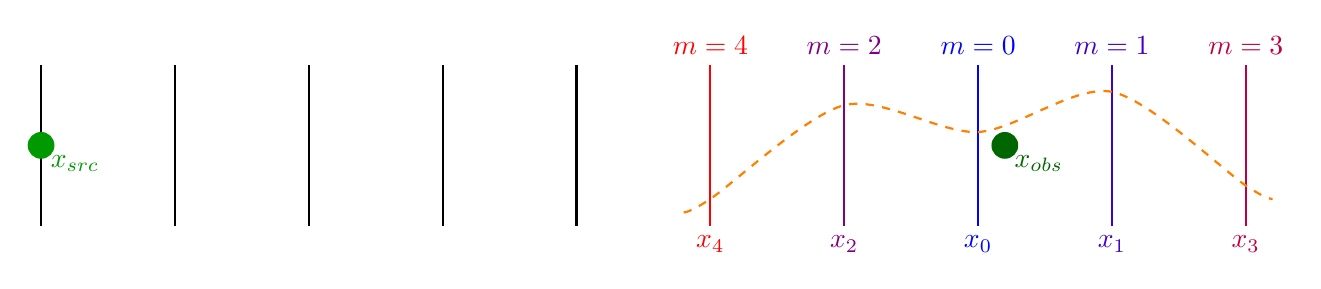
\begin{tikzpicture}[scale=1.7]

\foreach \i in {0, ..., 4}
{
  \draw[thick] (\i, -0.6) -- (\i, 0.6);
}

\fill[green!60!black] (0,0) circle (0.1) node [anchor=north west] {$x_\text{src}$};
\fill[green!40!black] (7.2,0) circle (0.1) node [anchor=north west] {$x_\text{obs}$};

\draw[thick, blue] (7,-0.6) node[below]{$x_0$} -- (7, 0.6) node[above]{$m = 0$};
\draw[thick, blue!75!red] (8,-0.6) node[below]{$x_1$} -- (8, 0.6) node[above]{$m = 1$};
\draw[thick, blue!50!red] (6,-0.6) node[below]{$x_2$} -- (6, 0.6) node[above]{$m = 2$};
\draw[thick, blue!25!red] (9,-0.6) node[below]{$x_3$} -- (9, 0.6) node[above]{$m = 3$};
\draw[thick, blue!0!red] (5,-0.6) node[below]{$x_4$} -- (5, 0.6) node[above]{$m = 4$};

\draw[dashed, thick, orange, mark position=0.9(g)] plot [smooth] coordinates {(4.8, -0.5) (5,-0.4) (6, 0.3) (7, 0.1) (8, 0.4) (9, -0.3) (9.2, -0.4)};
%\node[orange, anchor=west] (g) at (9.2, -0.4) {$g(x-x_\text{src})$};

\end{tikzpicture}
